\subsection{Model Implementation}

Code can be found in the attachments.

\subsection{Simulation}

4-Bit Adder

\begin{center}
    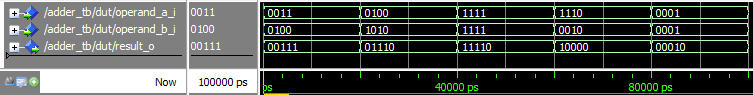
\includegraphics[width=\textwidth]{images/Adder4Sim.png}
\end{center}

12-Bit Adder

\begin{figure}[h]
    \centering
    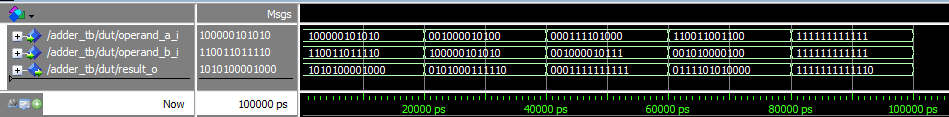
\includegraphics[width=\textwidth]{images/Adder12Sim.png}
    \caption{Caption}
    \label{fig:}
\end{figure}

Die Bitbreite der operanden ist \vhdl{BITWIDTH-1 downto 0} sodass die Breite inklusive der null genau der Bitbreite entspricht. Im Fall des 4-Bit Adder also von 3 bis 0. Beim Ausgang soll das Carry-Bit berück-sichtigt werden, damit die Zahl dargestellt werden kann wenn das Ergebnis die Bitbreite überschreitet. Die größe des resultates ist beim Addierer maximal 1 Bit größer als der größte Eingangswert. Die dimension des resultates ist daher \vhdl{BITWIDTH downto 0}.


Als Testwerte wurden Zahlen verwendet, die unterschiedliche Auswirkungen auf das Carry-Bit haben. Bei der 4-Bit Adder Simulation ist gut zu sehen, wie für beide operanden der höchste 4-Bit Wert 15 gewählt wurde. Wie man sieht, bleibt das resultat innerhalb des definierten Bit-Bereiches
